\section{Clase 5. Volumen de un prisma rectangular}\label{chap:C5}
\textbf{18/02/2025}

La clase comenzó con la realización de un trapecio rectangular por medio de origami y los pasos fueron los siguientes:
\begin{itemize}
    \item Doblar la hoja del punto $A$ al punto $Q$
    \item Doblar la hoja del punto $B$ al punto $P$
    \item Doblar la hoja del punto $D$ de al punto $P'$
    \item Doblar la hoja del punto $C$ al punto $Q'$
\end{itemize}

De modo que sobre la hoja queden las siguientes marcas:

\begin{figure}[h!]
    \caption{Representación de la hoja sobre la cual se trabajó}
    \begin{center}
        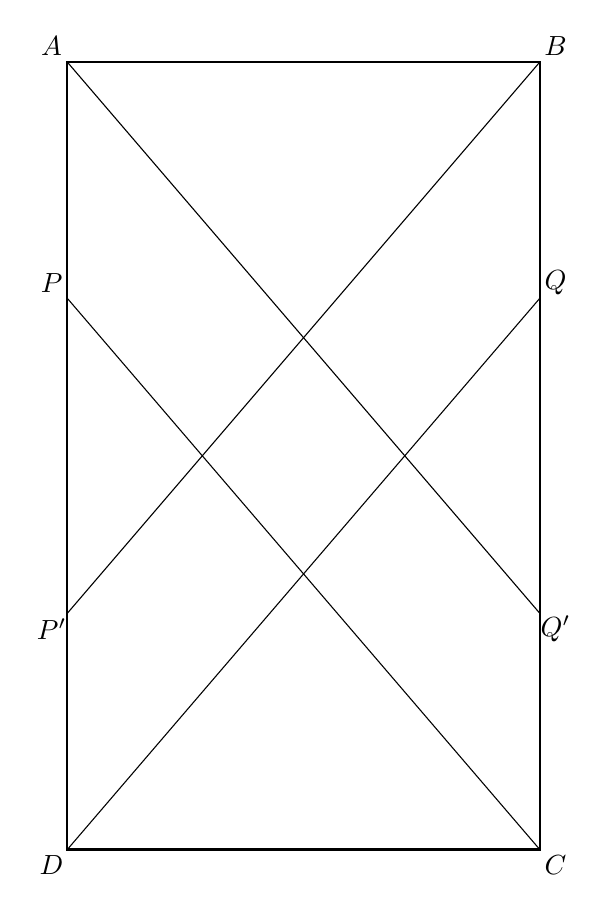
\begin{tikzpicture}
            % Dibujar el rectángulo (hoja)
            \draw[thick] (-3,5) -- (3,5) -- (3,-5) -- (-3,-5) --cycle;
            \node at (-3.2,5.2) {\textbf{$A$}};
            \node at (3.2,5.2) {\textbf{$B$}};
            \node at (3.2,-5.2) {\textbf{$C$}};
            \node at (-3.2,-5.2) {\textbf{$D$}};
            
            \draw[thin] (3,-5) -- (-3,2);
            \node at(-3.2,2.2){\textbf{$P$}};
            \draw[thin] (3,2) -- (-3,-5);
            \node at(3.2,2.2){\textbf{$Q$}};
            
            \draw[thin] (3,-2) -- (-3,5);
            \node at(-3.2,-2.2){\textbf{$P'$}};
            \draw[thin] (3,5) -- (-3,-2);
            \node at(3.2,-2.2){\textbf{$Q'$}};
        \end{tikzpicture}
    \end{center}
\end{figure}

Luego deben unirse los siguientes puntos: 

\begin{itemize}
    \item $A$ y $B$
    \item $C$ y $D$
    \item $P'$ y $P$
    \item $Q'$ y $Q$
\end{itemize}
Y hacer los dobleces de la hoja hacia adentro de modo que quede algo similar a esto:

\begin{center}
    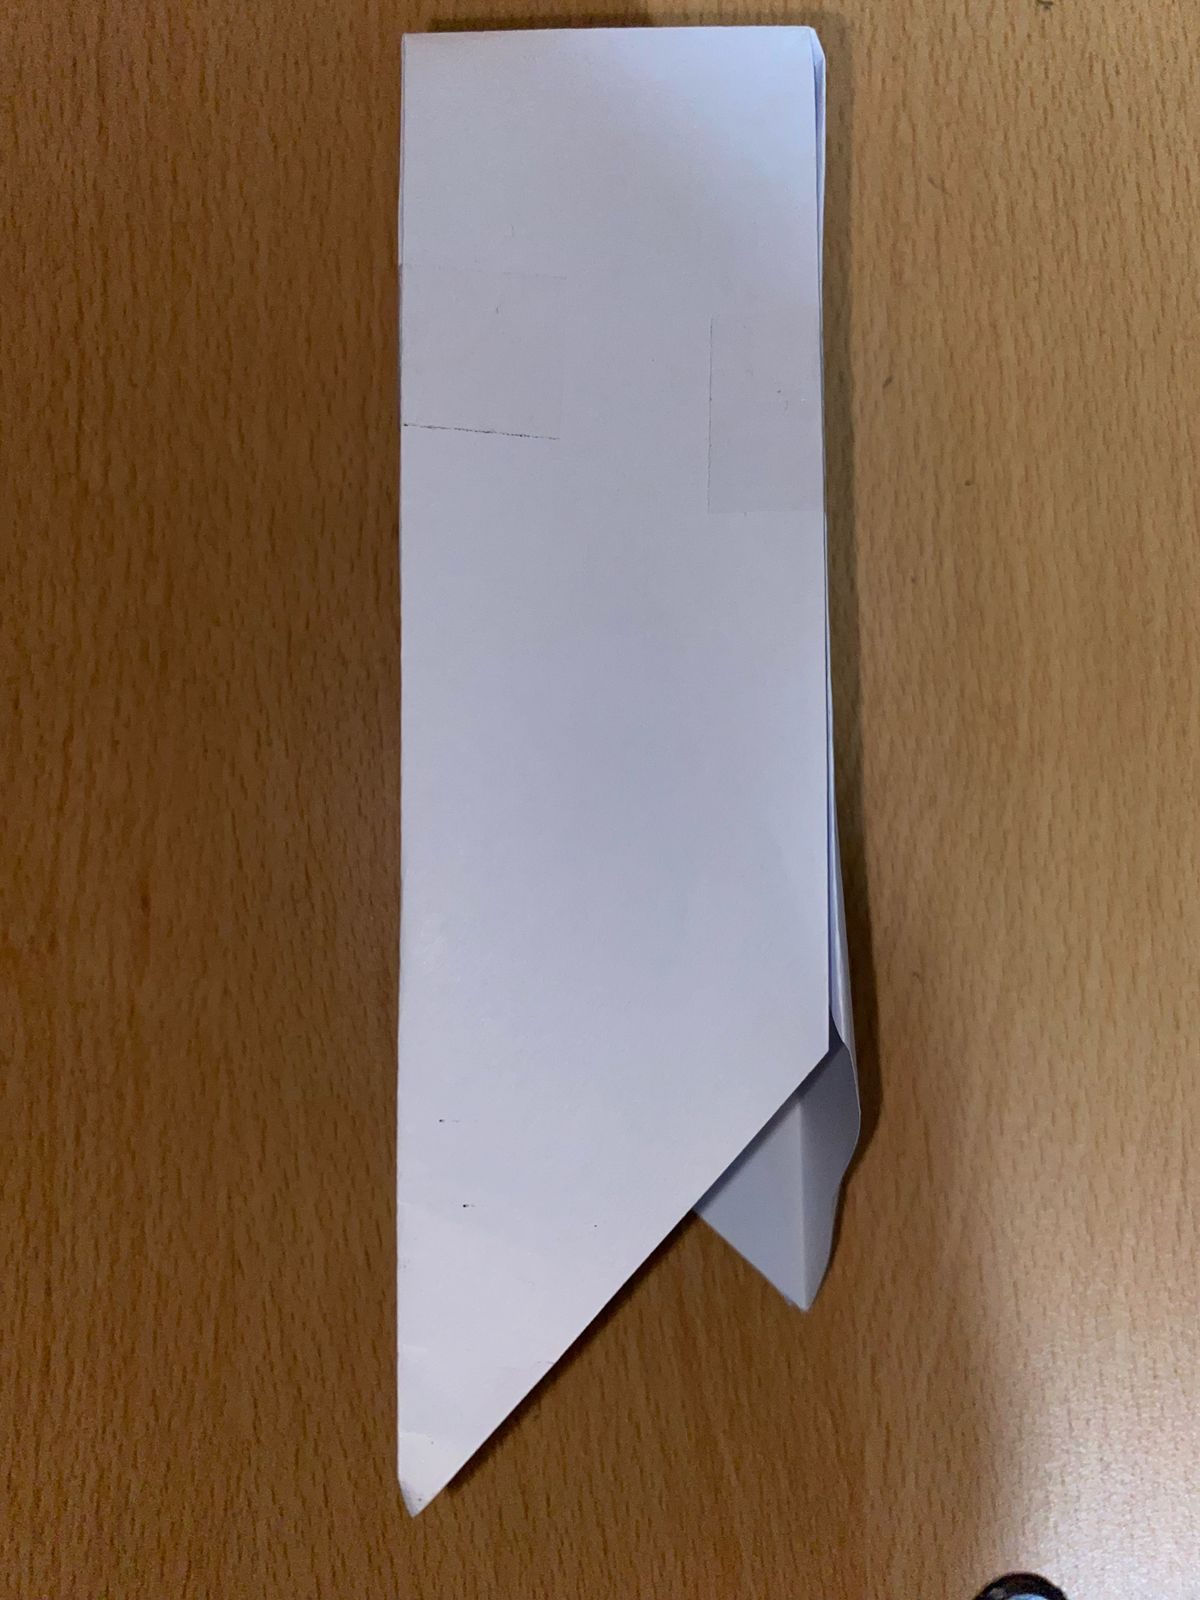
\includegraphics[scale=0.1]{clase5/semiTrapecio.jpeg}
\end{center}

Despues se doblan las puntas, de modo que quede el prisma de la siguiente forma.

\begin{center}
    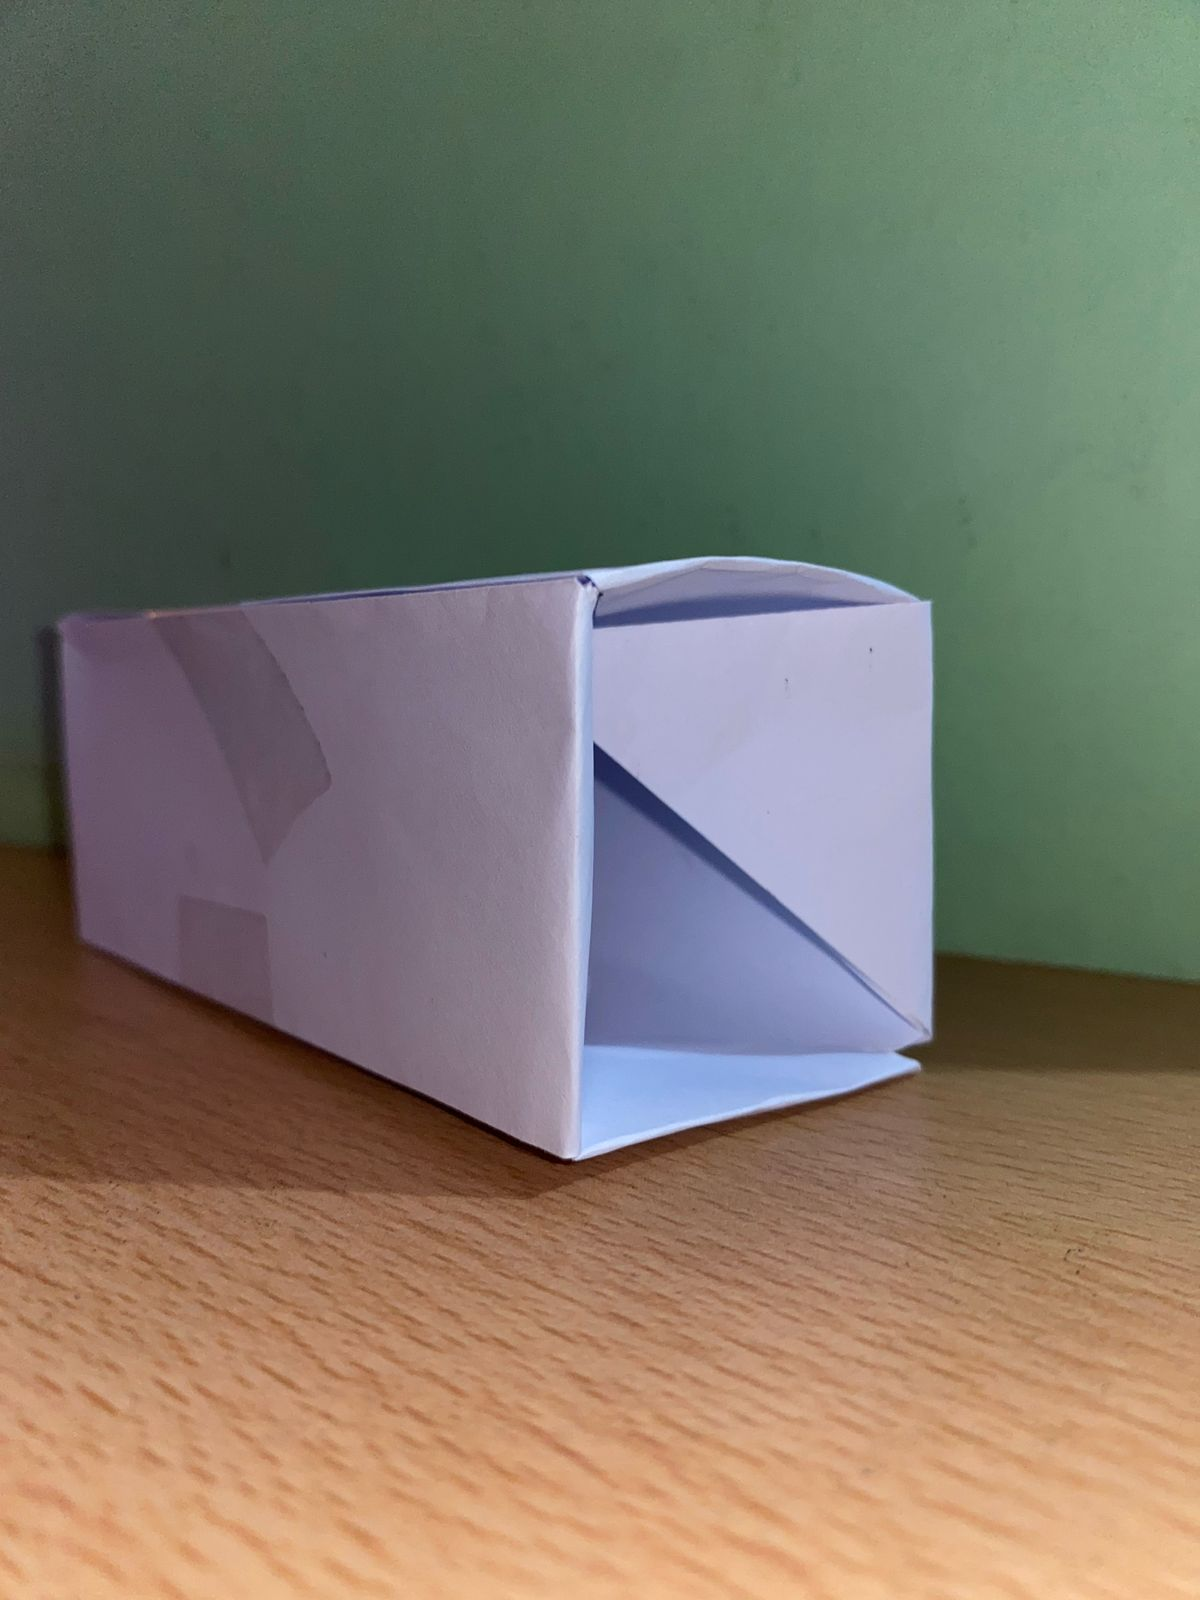
\includegraphics[scale=0.09]{clase5/trapecioFin.jpeg}
\end{center}

Y se hace uno similar para un cuarto del tamaño de la hoja
\begin{figure}[ht!]
    \begin{center}
        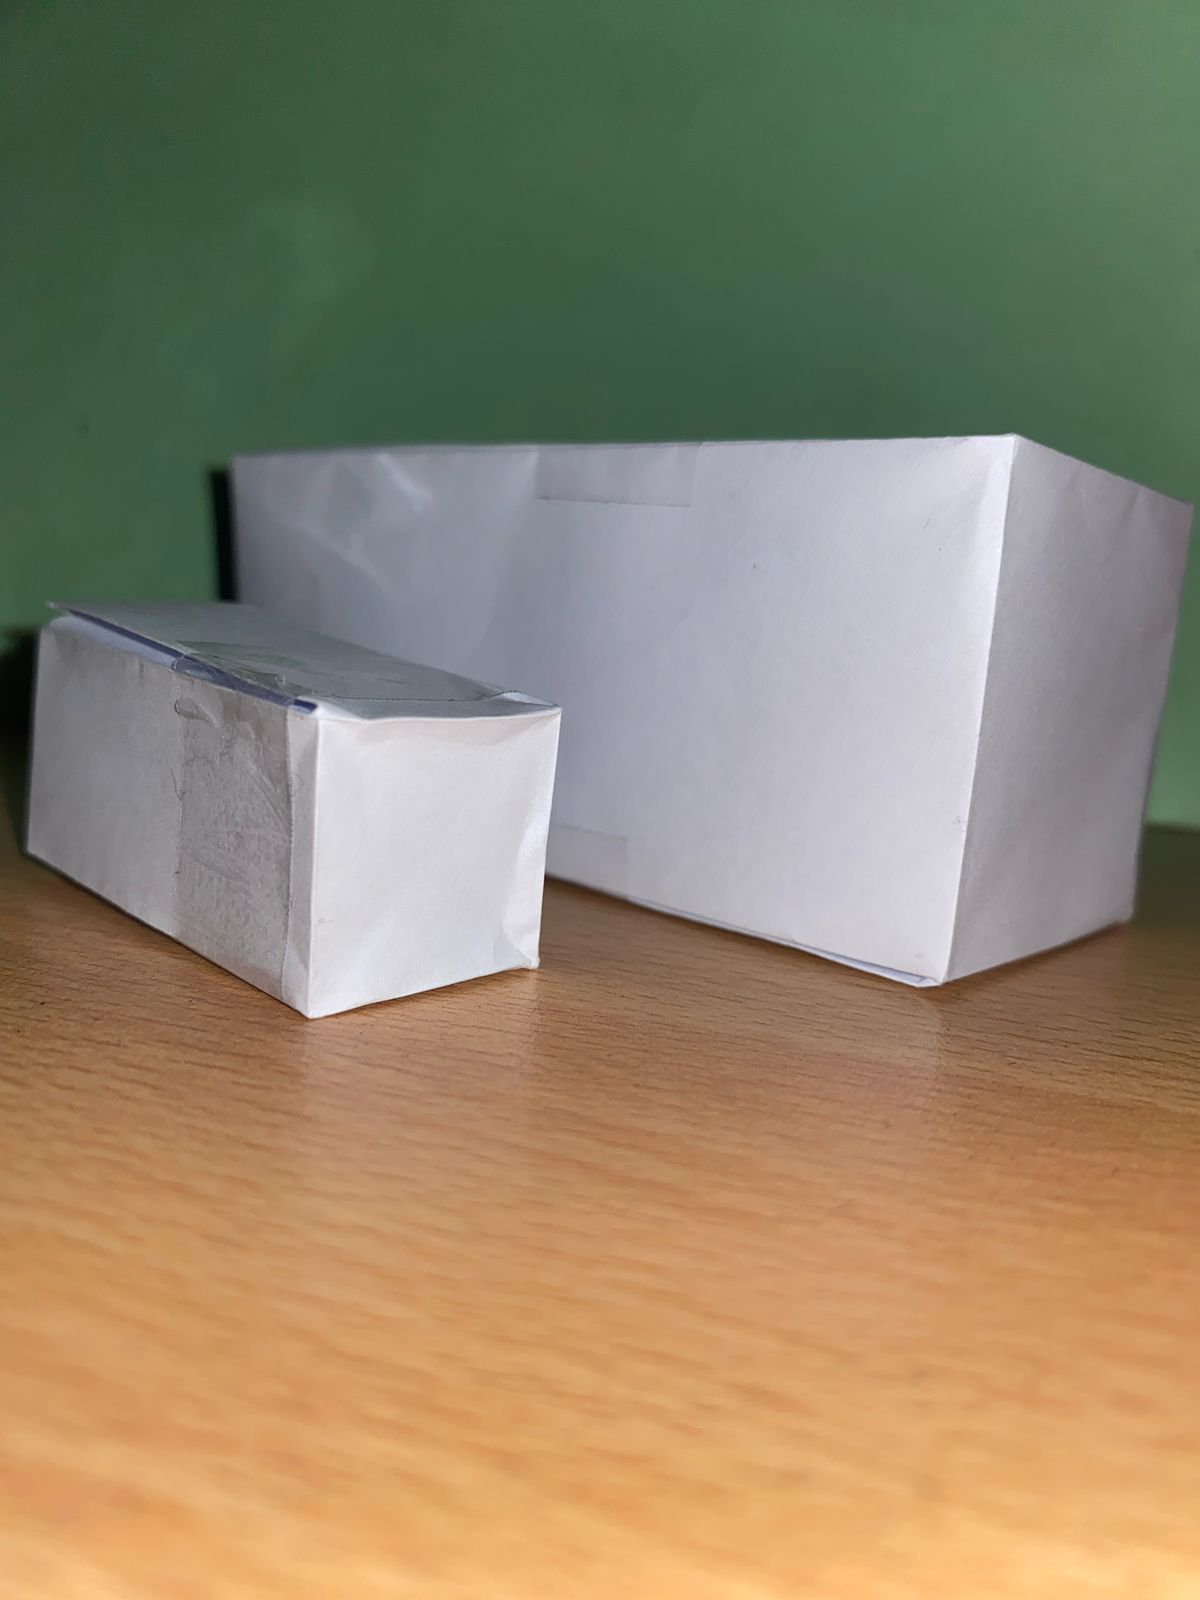
\includegraphics[scale=0.09]{clase5/prismaPyG.jpeg}
    \end{center}
\end{figure}

Durante la actividad la primera pregunta fue ¿Cuántos prismas pequeños caben en el prisma grande? Nuestra respuesta como equipo fue 4, pero luego sacando el volumen del prisma grande y de un prisma pequeño, nos dimos cuenta de que cabían 8

\textbf{¿Cómo encontramos la fórmula para el volumen de un prisma pequeño?}

Primero medimos la altura de los prismas y buscamos encontrar alguna proporción, la cual fue de $\frac{1}{2}$ de cualquiera de las medidas del prisma grande al prisma pequeño y posterior a eso surgió la idea ilustrada abajo. 

\begin{figure}[ht!]
    \begin{center}
        \begin{tikzpicture}
            % Proporciones normales
            \draw[thick] (-5,5) -- (-2,5) -- (-2,0) -- (-5,0) --cycle;
            \draw[<->] (-5,-0.5) -- (-2,-0.5);
            \node at (-3.5,-0.8) {\textbf{$x$}};
            \draw[<->] (-1.5,0) -- (-1.5,5);
            \node at (-1,2.5) {\textbf{$y$}};
            
            % Proporciones reducidas
            \draw[thick] (0,5) -- (3,5) -- (3,0) -- (0,0) --cycle;
            % Dividiendo la hoja en 4 partes
            \draw[dashed] (1.5,5) -- (1.5,0);
            \draw[dashed] (0,2.5) -- (3,2.5);
            % Flechas reducidas
            \draw[<->] (1.5,-0.5) -- (3,-0.5);
            \node at (2.4,-0.8) {\textbf{$\frac{x}{2}$}};
            \draw[<->] (3.5,0) -- (3.5,2.5);
            \node at (3.8,1.5) {\textbf{$\frac{y}{2}$}};
        \end{tikzpicture}
    \end{center}
    \caption{Aunque el material usado se redujo a un cuarto, la medida del largo y del ancho solo se redujeron a la mitad}
\end{figure}

Después de esto solo trabajamos sobre la fórmula para calcular el volumen de un prisma rectangular:

\begin{gather*}
    f(x) =  V_G \\
    V_G = lah \qquad \text{Donde $l$: largo, $a$: ancho y $h$: altura } \\
    V_p = \frac{l}{2} \cdot \frac{a}{2} \cdot \frac{h}{2}\\
    V_p = \frac{lah}{8}\\
    V_p = \frac{V_G}{8}\\
    V_p \cdot 8= V_G
\end{gather*}
